\documentclass[12pt]{article}
\usepackage{times}
\usepackage[english]{babel}
\usepackage[utf8x]{inputenc}
\usepackage[colorinlistoftodos]{todonotes}
\usepackage[margin=1in]{geometry}
\usepackage{graphicx}
\usepackage{epstopdf}
\usepackage{cite}
\usepackage{listings}
\usepackage{dtklogos}
\usepackage{wrapfig}
\usepackage{subfigure}
\usepackage{amsmath}
\usepackage{amsthm}
\usepackage{amssymb}
\usepackage{amscd}
\usepackage{caption}
\usepackage{etoolbox}
\usepackage{fancyhdr}
\usepackage{stackengine}
\usepackage[export]{adjustbox}
\patchcmd{\thebibliography}{\section*{\refname}}{}{}{}
\usepackage[document]{ragged2e}    %This causes text to left align
\usepackage[colorlinks=true, linkcolor=black,citecolor=black,urlcolor=blue]{hyperref}
\bibliographystyle{IEEEtran}
\DeclareGraphicsRule{.tif}{png}{.png}{`convert #1 `dirname #1`/`basename #1 .tif`.png}

\title{MCHE 220: Report 4}

\begin{document}
\lefthyphenmin3
\righthyphenmin4
% \pretolerance=2000
% \tolerance=500 
% \emergencystretch=10pt
%\raggedright     %Stops LaTeX from automatically hyphenating the right margin to fit better
%Combine this with \usepackage[document]{ragged2e} to get a text align left similar to natural MS Word
%-------------------------------------------------------------
%Header
%-------------------------------------------------------------
\fancyhf{}  
  \renewcommand{\headrulewidth}{0pt}
  \fancypagestyle{plain}{
    \fancyhead[R]{\thepage}} 
    \pagestyle{plain}
    
\captionsetup[table]{labelsep=space}

\begin{flushleft}
\hrulefill\\\hrule height 1pt
\vspace{5pt}
\textbf{TO: }William J. Emblom, Ph.D.  \hfill   \textbf{DATE: }\today                
\bigskip\\
\textbf{FROM: }Matthew J. Begneaud
\bigskip\\
\textbf{COPY: }N/A
\bigskip\\
\textbf{RE: }MCHE 220 Lab 4
\vspace{-10pt}
\end{flushleft}
\hrulefill \hrule height 1pt

%-------------------------------------------------------------
%Start of Paper
%-------------------------------------------------------------

\section*{\fontsize{12}{12}\selectfont INTRODUCTION}
This memorandum is being sent to Dr. Emblom to convey the analysis of a creep test which took place on campus at University of Louisiana at Lafayette. The test was performed on a length of solder by hanging it from a hook and then hanging a weight from the bottom end of the solder. A gauge length measurement was taken periodically until the solder failed. The results of the test will be shown, as well as multiple data plots recorded and calculated from the experiment. These plots will be used to analyze the meaning of the data.
\bigskip



\section*{\fontsize{12}{12}\selectfont BACKGROUND}
The data collected from the test include the time of each measurement, as well as the measurement of the top and bottom gauge marks, which will be used to obtain the length between the marks. The original diameter of the solder and the mass of the weight are also recorded. Using the given data, the engineering stress and strain are both calculable. The engineering stress is defined as the force applied on an object divided by the original area of the face the force is applied normal to, as shown in (1). The engineering strain is defined as the change in length of an object per unit-length, as shown in (2).

\bigskip
\begin{equation}
\sigma_{E} = \frac{F}{A_{o}}
\end{equation}
\bigskip


\begin{equation}
\epsilon = \left | \frac{l_{o}-l}{l_{o}} \right |
\end{equation}
\bigskip

Using the given data, the solder's cross-sectional area at any point of the test is calculable by relating the volume to the change in length and solving for the new corresponding area, resulting in (3). True stress, which is defined as the force applied to an object divided by the instantaneous area of the face the force is applied normal to, is calculable by (4). True strain is also calculable with the given data. According to [1], true strain is found by integrating the rate of the deformation tensor with respect to time, which results in (5).

\begin{equation}
A = \frac{l_{o}}{l}A_{o}
\end{equation}
\bigskip

\begin{equation}
\sigma_{T} = \frac {F}{A}
\end{equation}
\bigskip

\begin{equation}
\phi = \left | ln \frac{l}{l_{o}} \right |
\end{equation}
\bigskip

According to [2], the tendency of an object to deform over time due to being stressed at high temperatures is referred to as creep. In situations where the temperature is high, though not close to the melting temperature, a metal object can become weak and start to deform easily, which means as the temperature gets higher, the creep will also get higher for the object. Creep is analogous to elasticity, which is proportional to the strain since it is also defined as the tendency to elongate; therefore strain is used to measure creep. Note that since strain is a change in length per unit length, the original length of the material does not effect either the strain or the creep. A different area would not effect the strain or creep either, since area is not a variable in calculating strain, as seen in (5).
\bigskip

Zones on a creep curve can also be split into three different zones: the primary zone, secondary zone, and the tertiary zone. These zones will be shown in the Results and Discussion section. The primary zone is when the curve is rising up to the yield point with a decreasing slope. The secondary zone is when the curve tends to reach a steady slope. The tertiary zone is where the slope of the curve starts to become flat again.
\bigskip



\section*{\fontsize{12}{12}\selectfont PROCEDURE}
The creep test was conducted in the metal forming lab on campus. The equipment used was a weight of 4.82 kg, a strip of metal solder, metal hooks, and a yard stick. The strip of solder was hung on the wall in front of the yard stick and the weight was hung on the bottom end of the solder. Before hanging the weight, two gauge marks were made on the solder spaced apart at an original length of 7 inches. This configuration can be seen in Figure 1. 
\bigskip

The measurement time interval for the first and third creep zones should be small in order to capture the primary and tertiary zones of the curve well in the data, while the secondary creep zone does not require as many data points to give an accurate depiction. After hanging the weight from the solder, the length between the gauge marks was measured every 10 seconds for 260 seconds, and then measurements were taken every 60 seconds. The time period was to switch back to 10 seconds to capture the tertiary curve well, but the solder snapped unsuspectingly early. 

\newpage

\begin{figure}[htbp] %  figure placement: here, top, bottom, or page
   \centering
   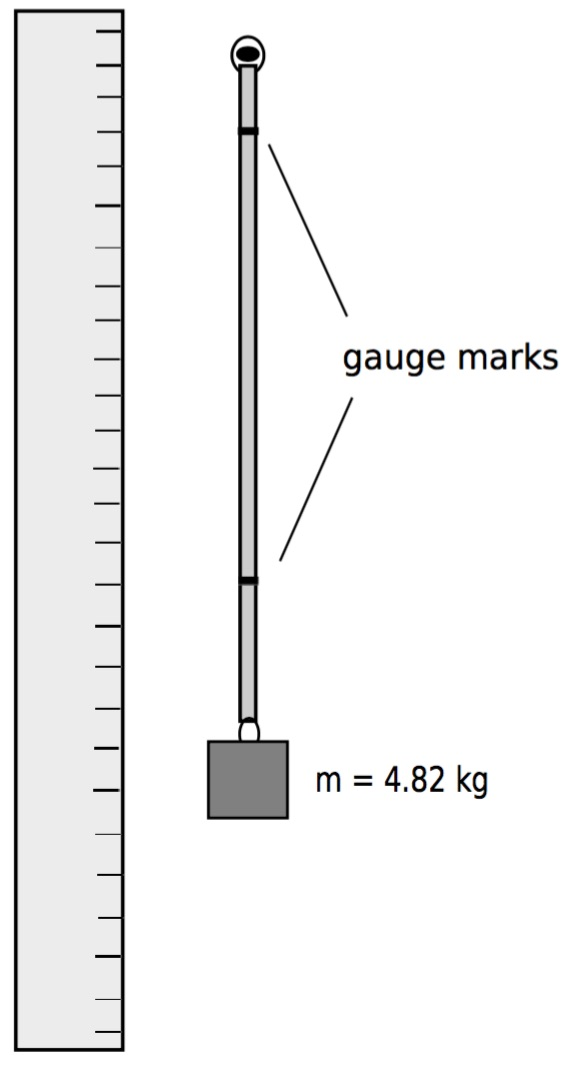
\includegraphics[width=2in]{experiment_setup.jpg} 
   \caption{Experiment Setup}
\end{figure}
\bigskip


The recorded data includes the mass of the weight, the time at which measurements took place, and the distance between the gauge marks at each measurement. This data was then used to calculate the engineering stress and strain, as well as the true stress and strain. The engineering and true strain were both plotted versus time on the same graph and the primary, secondary, and tertiary zones were identified on the plot. The true strain was then plotted versus time again on a log-log graph. The true stress was also plotted against time. Note that the engineering stress is not plotted versus time because the engineering stress remains constant throughout the experiment. This is because the engineering stress only relies on force and original area, seen in (1), and the force remains constant in this experiment.
\bigskip



\section*{\fontsize{12}{12}\selectfont RESULTS AND DISCUSSION}
The data recorded from the experiment is shown in Table 1. A plot of the engineering and true strain versus time is shown in Figure 2. It can be seen from the plot that the engineering strain results in an overestimation of the real value by comparing it to the true strain. The three main zones of creep are also identified in the plot. 

\newpage

% table1
\begin{center}
Table 1 

\emph{Creep Test of Solder}

\begin{tabular}{ c c c c c c}
\hline
Force & Length & Area & Engineering Strain & True Strain & True Stress\\
(s) & (mm) & (mm$^2$) & --- & --- & (MPa)\\
\hline
0    & 177.80 & 7.92 & 0.0000 & 0.0000 & 5.972 \\
10   & 177.80 & 7.92 & 0.0000 & 0.0000 & 5.972 \\
20   & 180.98 & 7.78 & 0.0179 & 0.0177 & 6.079 \\
30   & 184.15 & 7.64 & 0.0357 & 0.0351 & 6.186 \\
40   & 184.15 & 7.64 & 0.0357 & 0.0351 & 6.186 \\
50   & 184.15 & 7.64 & 0.0357 & 0.0351 & 6.186 \\
60   & 185.74 & 7.58 & 0.0446 & 0.0437 & 6.239 \\
70   & 185.74 & 7.58 & 0.0446 & 0.0437 & 6.239 \\
80   & 185.74 & 7.58 & 0.0446 & 0.0437 & 6.239 \\
90   & 187.33 & 7.51 & 0.0536 & 0.0522 & 6.292 \\
100  & 187.33 & 7.51 & 0.0536 & 0.0522 & 6.292 \\
110  & 188.91 & 7.45 & 0.0625 & 0.0606 & 6.346 \\
120  & 188.91 & 7.45 & 0.0625 & 0.0606 & 6.346 \\
130  & 188.91 & 7.45 & 0.0625 & 0.0606 & 6.346 \\
140  & 188.91 & 7.45 & 0.0625 & 0.0606 & 6.346 \\
150  & 190.50 & 7.39 & 0.0714 & 0.0690 & 6.399 \\
160  & 190.50 & 7.39 & 0.0714 & 0.0690 & 6.399 \\
170  & 190.50 & 7.39 & 0.0714 & 0.0690 & 6.399 \\
180  & 190.50 & 7.39 & 0.0714 & 0.0690 & 6.399 \\
190  & 190.50 & 7.39 & 0.0714 & 0.0690 & 6.399 \\
200  & 193.68 & 7.27 & 0.0893 & 0.0855 & 6.505 \\
210  & 193.68 & 7.27 & 0.0893 & 0.0855 & 6.505 \\
220  & 193.68 & 7.27 & 0.0893 & 0.0855 & 6.505 \\
230  & 194.31 & 7.24 & 0.0929 & 0.0888 & 6.527 \\
240  & 194.63 & 7.23 & 0.0946 & 0.0904 & 6.537 \\
250  & 195.67 & 7.19 & 0.1005 & 0.0958 & 6.572 \\
260  & 200.34 & 7.03 & 0.1268 & 0.1194 & 6.729 \\
320  & 201.61 & 6.98 & 0.1339 & 0.1257 & 6.772 \\
380  & 204.79 & 6.87 & 0.1518 & 0.1413 & 6.879 \\
440  & 206.38 & 6.82 & 0.1607 & 0.1490 & 6.932 \\
500  & 206.38 & 6.82 & 0.1607 & 0.1490 & 6.932 \\
560  & 211.14 & 6.67 & 0.1875 & 0.1719 & 7.092 \\
620  & 211.14 & 6.67 & 0.1875 & 0.1719 & 7.092 \\
680  & 212.73 & 6.62 & 0.1964 & 0.1793 & 7.145 \\
740  & 212.73 & 6.62 & 0.1964 & 0.1793 & 7.145 \\
800  & 220.66 & 6.38 & 0.2411 & 0.2160 & 7.412 \\
860  & 220.66 & 6.38 & 0.2411 & 0.2160 & 7.412 \\
920  & 220.66 & 6.38 & 0.2411 & 0.2160 & 7.412 \\
\hline
\end{tabular}

\newpage

Table 1 (cont.) 


\emph{Creep Test of Solder} 


\begin{tabular}{ c c c c c c}
\hline
Force & Length & Area & Engineering Strain & True Strain & True Stress\\
(s) & (mm) & (mm$^2$) & --- & --- & (MPa)\\
\hline

980  & 220.66 & 6.38 & 0.2411 & 0.2160 & 7.412 \\
1040 & 220.66 & 6.38 & 0.2411 & 0.2160 & 7.412 \\
1100 & 223.84 & 6.29 & 0.2589 & 0.2303 & 7.519 \\
1160 & 223.84 & 6.29 & 0.2589 & 0.2303 & 7.519 \\
1220 & 215.90 & 6.52 & 0.2143 & 0.1942 & 7.252\\
\hline
\end{tabular}
\end{center}
\bigskip


\begin{figure}[htbp] %  figure placement: here, top, bottom, or page
   \centering
   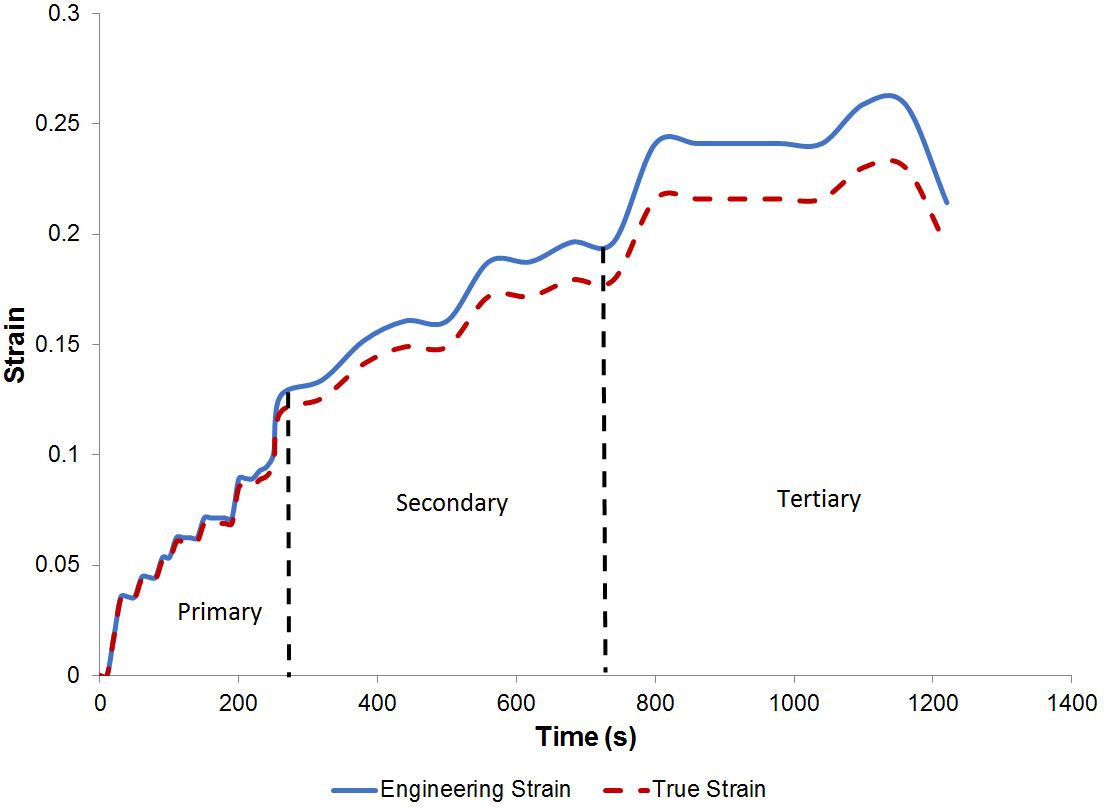
\includegraphics[width=\linewidth,height=4.4in]{creep_zones.jpg} 
   \caption{Engineering and True Strain vs Time}
\end{figure}
\bigskip


The true strain is plotted versus time again in Figure 3 on a log-log graph. It can be seen that the curve is closer to being linear than the true strain curve in Figure 2. This is because the slope of true strain is logarithmic in nature, as shown in (6), where B is the slope of the true strain curve. As seen in Table 1, the length measurement did not change from the original length at the 10 second measurement, which results in a strain of zero. The logarithmic plot in Figure 3 excludes the 0 and 10 second strain measurements because zero has no logarithm.
\bigskip


\begin{equation}
B = \frac{ln\sigma_{1}-ln\sigma_{2}}{ln\phi_{1}-ln\phi_{2}}
\end{equation}

\newpage

\begin{figure}[htbp] %  figure placement: here, top, bottom, or page
   \centering
   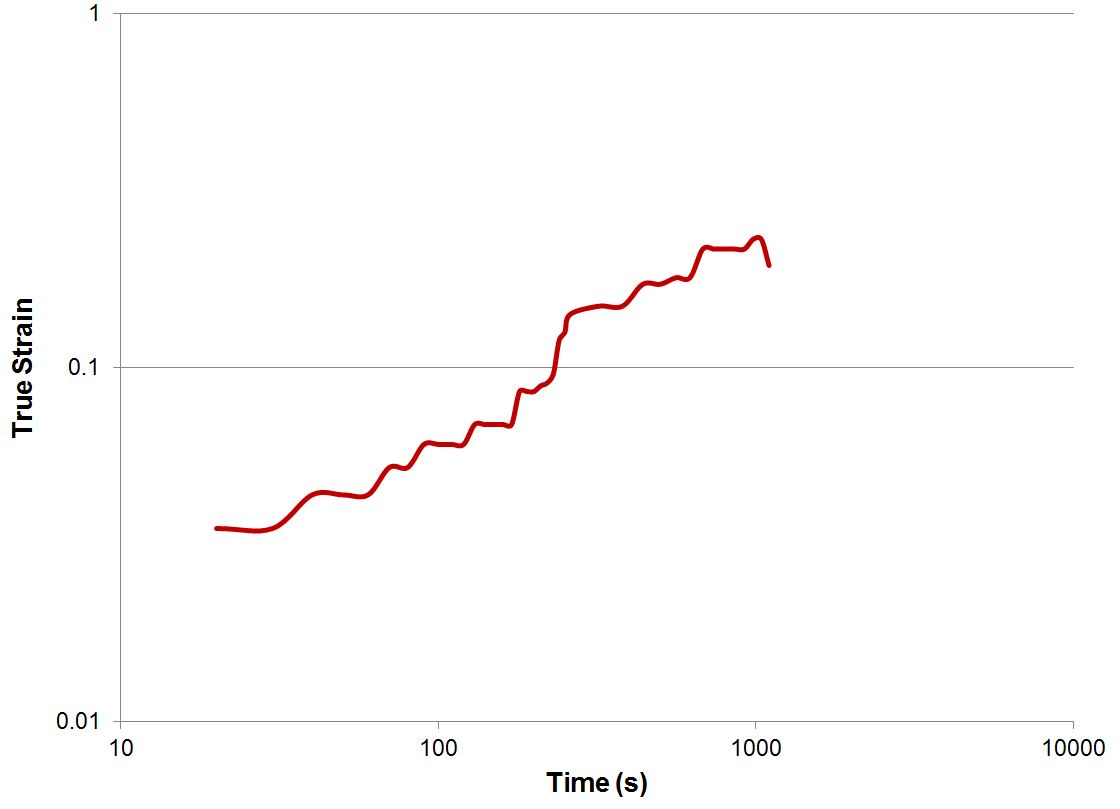
\includegraphics[width=\linewidth]{t_strain_vs_time_log.jpg} 
   \caption{True Strain vs Time (log-log scale)}
\end{figure}
\bigskip


The engineering stress, which remained constant throughout the experiment, was found to be 5.97 MPa. The true stress is also plotted against time in Figure 4. It can be seen in Figure 2 and Figure 4 that the solder gets stressed past its yield point around 300 seconds, where the curve begins to flatten out. Note that in all of the plots, the point of failure at the end of the curves follows the characteristic drop in stress and/or strain that occurs right before the material fails. It should also be noted that the data curves would be much smoother if measurements were taken much more frequently and by more accurate methods.
\bigskip

As discussed, the true stress and strain give more accurate values than the engineering stress and strain. This is because the change in area elements is considered in calculations. Since the two types of stress and strain behave similarly up to the yield point where deformation begins to occur, as shown previously in Figure 2, it is recommended that engineering stress and strain only be used for analysis regarding materials that are not loaded enough to cause any deformation. If deformation is likely to occur in the range of loading considered for a material, true stress and strain should be used. 

\newpage


\begin{figure}[htbp] %  figure placement: here, top, bottom, or page
   \centering
   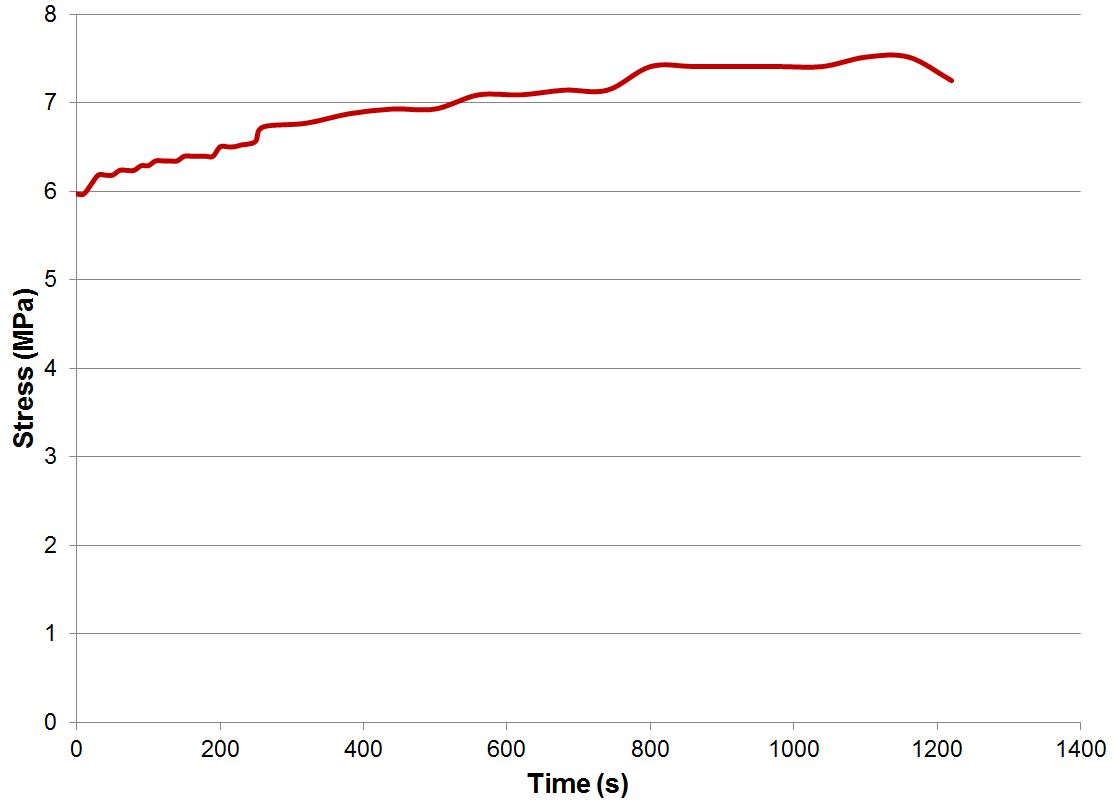
\includegraphics[width=\linewidth]{t_stress_vs_time.jpg} 
   \caption{True Stress vs Time}
\end{figure}
\bigskip


In respect to creep, this material would have stretched even easier and faster if it were exposed to much higher temperatures. This is because creep is proportional to temperature. As a material gets closer to its melting temperature, it becomes more elastic. According to [3], this is because heat adds energy to the metal's atoms, which allows them to more easily move past each other. The reason they can more easily move past each other is because the additional heat energy, combined with the stress on the metal, eventually becomes enough to overcome the molecular forces keeping the atoms in a fixed location. Each type of metal consists of different atoms, which require different amounts of energy to break out of their stationary positions. 
\bigskip

Solder has a very low melting temperature of about 183 degrees Celsius in order to suit its typical application in electronics, which results in being very susceptible to creep at relatively low stresses. Solder was used in this test because any other metal would typically have a much higher melting temperature and would have to be heated extensively before the weight used would cause failure. 
\bigskip

When designing any system, caution should be taken with choosing materials, especially in regards to creep. For example, if a system will be undergoing high temperatures, then any materials under load should have a melting temperature much higher than the temperatures they are exposed to. This will prevent these members of the system from deforming due to creep.

\newpage


\section*{\fontsize{12}{12}\selectfont CONCLUSION}
The data from this creep test performed on UL campus has been analyzed and plotted. The originally recorded data was also used to calculate the engineering and true strain, as well as the true stress. The results were plotted and it was found that the engineering strain was an overestimation of the real value when compared to the true strain. It was also observed that the data closely followed the fact that the slope of a true strain curve is linear in the logarithmic scale. 
\bigskip

In regards to creep, the experiment exhibited the fact that solder has a very high creep because it failed under relatively low stress at room temperature, whereas most metals have high melting temperatures and are not effected by creep until exposed to very high temperatures. This experiment exhibits that when designing a system, any load-bearing members should be made with materials that have high melting temperatures in order to mitigate the effects of creep.
\bigskip


\section*{\fontsize{12}{12}\selectfont REFERENCES}

\begin{thebibliography}{2}

\bibitem{McGinty}
Mcginty, B., n.d.,
"True Strain," \emph{Continuum Mechanics}, from
http://www.continuummechanics.org/

\bibitem{French}
French, D., July 1991,
"Creep and Creep Failures," from
http://www.nationalboard.org/Index.aspx?pageID=181

\bibitem{The Structure of Metals}
n.d., "Closest-Packed Structures," \emph{The Structure of Materials}, from
http://chemed.chem.purdue.edu/genchem/topicreview/bp/ch13/structure.php

\end{thebibliography}

%\section*{\fontsize{12}{12}\selectfont APPENDIX}

%\begin{table}[h!]
%  \caption{}
%  \includegraphics[width=\linewidth]{table1.png}
%\end{table}

\end{document}
----------------------------%TEmplates-------------------------------

-------------------------Figure-----------------------

\begin{figure}[h!]  
  \centering
    \includegraphics[width=\linewidth]{**file**}
    \caption{Docking Station}
\end{figure}

---------------------------Table-----------------------
\begin{table}[ht]
\caption{Nonlinear Model Results} % title of Table
\centering % used for centering table
\begin{tabular}{c c c c} % centered columns (4 columns)
\hline\hline %inserts double horizontal lines
Case & Method\#1 & Method\#2 & Method\#3 \\ [0.5ex] % inserts table
%heading
\hline % inserts single horizontal line
1 & 50 & 837 & 970 \\ % inserting body of the table
2 & 47 & 877 & 230 \\
3 & 31 & 25 & 415 \\
4 & 35 & 144 & 2356 \\
5 & 45 & 300 & 556 \\ [1ex] % [1ex] adds vertical space
\hline %inserts single line
\end{tabular}
\label{table:nonlin} % is used to refer this table in the text
\end{table}



probably best to insert as an image from excel

\bigskip\\
\begin{table}[h!]
  \caption{}
  \includegraphics[width=\linewidth]{**file**}
\end{table}
\bigskip\\





-----------------------------Equations------------------------
-----------------------------Regular
\begin{equation}
a = b + c
\end{equation}

--------------------------------- Multiline
\begin{multline}
a = b + c + d + e + f
+ g + h + i + j \\
+ k + l + m + n + o
\end{multline}

-------------------------------Citations-------------------------
\bibitem{Author last name}
  Last, First., year of publication,
  article name, book(etc) name, from \\
  link goes here

----------------------------------other-----------------------------

equations:
http://moser-isi.ethz.ch/docs/typeset_equations.pdf

citations:
http://library.missouri.edu/engineering/about/guides/asme
https://www.asme.org/shop/proceedings/conference-publications/references